% !TeX spellcheck = en_GB
\chapter{Methods}

In this section, I will discuss the setup I worked with and how we have characterised it. I will present the acquisition and analysis protocol I have developed to obtain polarisation microscopy images, and also introduce pSTED, a method to increase the resolution in the polarisation domain. Finally, I will discuss the samples I have used in this thesis.

\section{Microscope setup}

\begin{figure}[h!]
	\centering
	\includegraphics[width=\linewidth]{microscope layout.pdf}
	\caption{
		Schematic overview of the Tegenfeldt microscope. The sample is located in a microscope housing on the bottom right (outside this figure). FC1 and FC2 are swappable filter cubes. Half-wave and quarter-wave plates are denoted $ \lambda/2 $ and $ \lambda/4 $, respectively. Dashed lines represent the light path, except those that go to the TCSPC (those are digital connections). The waveplates in the pSTED module were not in the original setup, and were added as part of this project. See text for more details.
	}
	\label{fig:layout}
\end{figure}

\begin{figure}
	\centering
	\includegraphics[width=.75\linewidth]{microscope photo.jpg}
	\caption{
		Photo of the optical enclosure, in the same orientation as \autoref{fig:layout}. The pSTED module is not shown.
	}
	\label{fig:microscope photo}
\end{figure}

In short, the Tegenfeldt STED microscope is a scanning confocal fluorescence microscope constructed by Abberior Instruments GmbH (Germany). It features two excitation lasers (at 561~nm and 640~nm) and one depletion laser at 775~nm for two-channel confocal or STED microscopy. It also contains a time-correlated single photon counter (TCSPC) for fluorescence lifetime imaging microscopy (FLIM) and a highly sensitive photomultiplier tube (PMT). Refer to Figures \ref{fig:layout} and \ref{fig:microscope photo} for the layout of these optical elements. Samples are located inside an inverted Nikon microscope body (Ti-E, not shown in the figure) equipped with a piezo stage (M-687 PILine XY-stage system and P-736 PInano (Physik Instrumente) Z Microscope Scanner), a 60x, 1.4~NA oil immersion objective (Nikon Plan Apo) and a QUADScan beam scanner (Cambridge Technology).

I will address all laser lines as well as the detection module in detail, with a focus on characterising the light polarisation at different points in the microscope.

\subsection{The laser modules.} The fast-switching 561~nm laser is initially horizontally polarised, but the polarisation can be tuned by three waveplates in its path. The last one, a quarter-wave plate, is fixed in its rotation angle. In the standard mode of operation, excitation laser light should be circularly polarised to minimise resolution reduction due to lens distortion etc.~\cite{Harke2008}. In that mode, the (fast or slow) axis of the first quarter-wave plate should be aligned with the laser, such that it does not affect polarisation and the half-wave plate should be set such that it rotates the (linearly polarised) light to \ang{45} with respect to the second quarter-wave plate. See \autoref{tab:laser polarisation} for the polarisation characteristics in the calibration provided by Abberior. The 561~nm laser is quite well-calibrated. In circular polarisation, it reaches a $ \chi $ very close to perfectly circular (\ang{45}).

The 640 nm laser does not have fast-switching built in, so instead, the light is fed into the microscope through a polarisation-preserving optical fibre by an acousto-optical modulator (AOM). The AOM is a crystal in the beam path, in which sound waves can be generated by a piezo element. The standing sound wave creates a diffraction grating with a variable pitch, determined by the sound frequency. The sound frequency can be modulated such that the first-order diffracted beam is either sent into the fibre aperture or not. The rest of the beam path is very similar to the 561 module, but the calibration of the waveplates in this pathway is not as accurate. Refer to \autoref{tab:laser polarisation}. 

The depletion laser travels through an entirely different set of optics than the excitation lasers to generate a donut beam. First, it travels through a half-wave plate that aligns the polarisation to the SLM (spatial light modulator). This HWP is necessary because an SLM adds an arbitrary spatially patterned phase delay to incident light, but only to the component polarised along its active axis. It will not alter the phase of the orthogonally polarised component. Using the proper phase delay patterns, one can create any (diffraction-limited) image in the sample plane. In our case, that would be a donut shape. Then -- and I am ignoring the pSTED module for now, since that was not included in the original setup -- the beam travels through a half-wave plate to ensure circular polarisation in the sample plane (after going through a quarter-wave plate at \ang{45} to the QWP axes), just like the excitation lasers. This is done to ensure that the depletion efficiency does not depend on sample orientation and to avoid polarisation-dependent PSF distortion by lenses and other optics. The quality of the STED polarisation is similar to that of the 640 nm laser. Note that this is actually a significant result, as that means the donut beam is not isotropically polarised. It will be far more effective at quenching fluorophores oriented along \ang{40} than those at \ang{130}.

\begin{table}
	\centering
	\begin{tabular}{lSSSS}
		\toprule
		Laser source     & {$ I_\mathit{max} / I_\mathit{min} $} & {$ \chi_I $ (deg)} & {$ \chi_E $ (deg)} & {$ \psi $ (deg)} \\ \midrule
		561 nm, linear (\ang{0})  & 23.6                              & 2.42                               & 11.6                               & 0                                \\
		561 nm, circular & 1.14                              & 41.2                               & 43.1                               & 20                               \\
		640 nm, linear (\ang{0})  & 6.13                              & 9.25                               & 22.0                               & 0                                \\
		640 nm, circular & 1.59                              & 32.2                               & 38.5                               & 120                              \\
		775 nm, circular & 1.61                              & 31.8                               & 39.2                               & 40                               \\ 
		775 nm, linear & 5.47 & 10.6 & 23.1 & 0 \\ \bottomrule
	\end{tabular}
	\caption{
		Polarisation characteristics of the lasers. Shown are linearity $ I_\mathit{max} / I_\mathit{min} $, ellipticity $ \chi_E $ ($ \chi_I $) of the electric field (intensity), and ellipse orientation $ \psi $ (anti-clockwise angle between ellipse orientation and vertical axis in sample plane). This data is based on \autoref{fig:laser polarisation}, except the linear setting of the 775 nm laser. This required fitting new waveplates, as explained later (\autoref{sec:psted implementation}).
	}
	\label{tab:laser polarisation}
\end{table}

One more thing we can derive from this data (see \autoref{fig:laser polarisation}), is that the 640 laser needs to ramp up every time it is powered on, due to the lack of fast switching. This can be somewhat prevented by setting the laser to ``always on'', albeit at a power of 0\%. Furthermore, at low powers, the laser intensity may not be proportional to the power setting in software. Their actual relationship is shown in \autoref{fig:laser power}. If experiments need to be done at low power, a neutral density filter is required. This is luckily not the case for biological specimens with a low density of fluorophores.

Looking at the calibrations of the waveplates in the excitation modules (\autoref{fig:excitation waveplate calibration}), one can see that they move quite erratically, but they do work, as shown in \autoref{fig:laser polarisation}. This could be an effect of the automated calibration performed by Abberior. In the 561 nm calibration, for example, one can see that the QWP constantly flips between about \ang{30} and \ang{120}, which are \ang{90} apart. The calibration works, but the eccentricity of the polarisation ellipse depends on the orientation. In other words, for a more rigorous characterisation of the microscope, \autoref{tab:laser polarisation} should have an entry for every possible calibration setting.

Finally, I also measured the PSFs of the lasers, by scanning over a reflective gold bead and acquiring an image on the photomultiplier tube (PMT). These are shown in \autoref{fig:normal psfs}.

\subsection{The detection module.} The main detectors of the microscope are a set of avalanche photodiodes (APDs), but there is also a highly sensitive PMT right after the QWP on the microscope end. The PMT is usually used to measure the point spread functions of the lasers and to align them with each other. In normal operation, the light travels on to the detection waveplates, then through a pinhole wheel, passes filters and dichroic mirrors in the filter cube housings, and is finally reflected onto the APDs. The wheel contains pinholes of different sizes, which allows for choosing the trade-off between light collection and $ z $ resolution, depending on the quality of the sample. Different filter cubes are available with various bandpass filters, dichroic mirrors, and/or a polarising beam splitter (PBS).

The APDs show a slight polarisation sensitivity, of about 10\% of the maximum sensitivity (see \autoref{fig:apd pol sensitivity}). I measured this by exciting Tetraspec beads with the 561 laser set to circular excitation, such that the emission light is non-polarised. Then I placed a linear polariser behind the detection waveplates and measured their signal as a function of the polariser angle. It seemed like the beam moved depending on the incident polarisation, as aligning the APDs when the signal was minimal did help a little, but the imperfect circularity of the 561 laser may also play a role, as it is on the same order of magnitude. 

We did have some problems with the waveplates in the detection module. They can be controlled through Abberior's software suite (Imspector), but it is not clear if they are set up correctly. The calibration is based on a control angle that I will denote by $ \theta $. It would theoretically be possible for this setup to rotate polarised light of any orientation, since
\begin{equation}
	S_\hwp(\theta/2) S_\qwp(0) S_\qwp(0) = \mqty(\cos\theta & -\sin\theta \\ \sin\theta & \cos\theta ),
	\label{eq:detection waveplates}
\end{equation}
which is simply the rotation matrix $ R(\theta) $. The exact position of the quarter-wave plates does not matter, as long as they are aligned with each other. If the waveplates are at a angle $ \phi $ instead of 0, then this set of waveplates rotates the polarisation by an angle $ (\theta-2\phi) $ instead. 

It is unclear what goal the original calibration (see \autoref{fig:detection waveplate calibrations}) should serve. If we approximate the default calibration with a QWP at $ \theta $ and a HWP at 0, then the action of these waveplates would be
\begin{equation}
	S_\hwp(0)\cdot S_\qwp(\theta)\cdot S_\qwp(0) = 
		\mqty( \cos^2\theta + i\sin^2\theta & (1+i)\cos\theta\sin\theta \\
			   (-1+i)\cos\theta\sin\theta   & \cos^2\theta - i\sin^2\theta 
	    ).
\end{equation}

Therefore, I developed a new calibration. To do so, I first needed to establish at what angle the second quarter-wave plate would be aligned to the first one. I did this by placing a polariser in the sample holder (P1) and illuminating it with the top lamp, such that the light incident on the first quarter-wave plate was linearly polarised. Then I placed another polariser (P2) after that waveplate (i.e.~before the last two waveplates) that I rotated to assess the linearity of the polarisation there. I found the angle of P1 at which light was most circular after the first QWP and subsequently placed P2 after all waveplates to find the angle of the second QWP that would make the polarisation linear again. At this point, the QWPs should be aligned.

\begin{figure}[h]
	\centering
	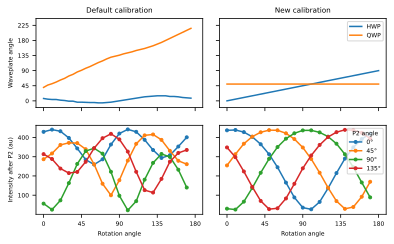
\includegraphics{detection_waveplate_calibrations.pdf}
	\caption{
		A comparison of the default detection waveplate calibration and the new one. The new calibration seems to actually rotate incident polarisation by an arbitrary angle.
	}
	\label{fig:detection waveplate calibrations}
\end{figure}


Second, I assessed both calibrations. As presented in \autoref{fig:detection waveplate calibrations}, my calibration works rather well, unlike the original one. However, its performance seems to depend on the precise angle of P1, see \autoref{fig:p1 effects}.
This needs to be fixed before we can confidently use polarisation-affecting elements in the detection path. Luckily, simulations show that this effect can be explained by misalignment between the QWPs. Therefore, a more accurate calibration should fix this problem.

\begin{figure}[h]
	\centering
	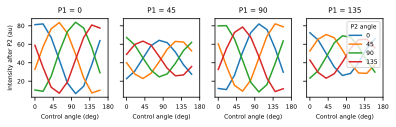
\includegraphics{p1_effects.pdf}
	\caption{
		The effect of rotating the incoming polarisation (P1). The detection waveplates seem to rotate the polarisation for P1 at \ang{45} or \ang{135}, but seem to circularise incoming light at \ang{0} and \ang{90} somewhat. (Note that the angle of P1 does not have a proper reference since I forgot to home the rotator.)
	}
	\label{fig:p1 effects}
\end{figure}

Finally, I checked the POL cube, which contains a polarising beam splitter (PBS) and some wavelength filters. It seems to work as expected (see \autoref{fig:pol cube}). The transmitted ray has an extinction ratio of about 0.2, meaning that 20\% of the power of rays that are orthogonally polarised to the transmission axis (and hence should be reflected by the PBS) is actually transmitted. On the other hand, it has an extinction ratio of .01 for the reflected wave.

\section{Conventional polarisation microscopy: acquisition and analysis}
\label{sec:pol analysis}
 
Because the current setup offers so much control over the light polarisation on both the excitation and detection ends, one can perform polarisation microscopy in several different ways:
\begin{enumerate}
	\item Measuring the intensity of emission components parallel and orthogonal to linearly polarised excitation ($ I_\parallel $ and $ I_\perp $). This is a very established method of polarisation microscopy, and allows for making anisotropy images, where every pixel is calculated according to
	\begin{equation}
		r=\frac{I_\parallel - I_\perp}{I_\parallel + 2I_\perp}.
	\end{equation}
	
	\item Detection of emission polarised at different angles after circularly polarised (or non-polarised) excitation.
	
	\item Detection of total emission intensity as a function of the polarisation angle of excitation light.
\end{enumerate}

Methods 1 and 2 require the POL cube to be placed in one of the filter cube housings. When placed in FC1, the POL cube reflects $ s $-polarised light (vertical) into APD1 and transmits $ p $-polarised light (horizontal) to be collected by APD2. Unfortunately, we cannot use these methods yet, since they rely on the action of the detection waveplates, even if they are not actively used during the acquisition. Once we do, however, the waveplates can be used to sample more than two angles during an acquisition. This is necessary to distinguish between light polarised along \ang{+-45}, since these two angles give exactly the same intensity when sampling at \ang{0} and \ang{90} degrees.

The last method, however, is not subject to those constraints, and is already achievable on the Tegenfeldt microscope. I have carried out some measurements and wrote code to analyse that data. The process of acquiring and analysing these images goes as follows:
\begin{enumerate}
	\item Acquire a stack of images at different excitation polarisation angles $ \theta_n $, resulting in a three-dimensional array of intensity values $ I_{nxy} $.
	\item Align images in this stack with each other, as the excitation beam seems to move as a function of polarisation angle. The alignment algorithm will be explained later.
	\item Compensate for photobleaching.
	\item For every pixel, calculate the Fourier coefficient corresponding to a \ang{180}-periodic signal.
	\item Based on that information, construct a new image in the HSV (hue, saturation, value) colour space where pixel colour depends on the polarisation direction, the saturation shows the degree of polarisation and the brightness (value) shows the total intensity of a pixel. 

\end{enumerate}

\subsection{Stack alignment.} Images in a stack are aligned using an ECC (enhanced correlation coefficient) optimisation algorithm implemented in OpenCV, an open source computer vision library, which optimises an adjusted version of the correlation between two images, subject to certain constraints, e.g.~translation, without shearing or rotation \cite{Evangelidis2008}. When the correlation between two images is maximised, they are aligned. The innovation of the ECC algorithm lies in the definition of an enhanced correlation coefficient which requires less computational power and is more robust than other algorithms \cite{Evangelidis2008}. 

If the goal is to generate a new image stack $ I'_{nxy} $, corrected for sample or beam drift, we can take the first frame as reference, setting 
\begin{equation}
	I'_{0xy} = I_{0xy}.
\end{equation}
For every other frame $ I_{nxy} $, we can calculate a warp matrix using OpenCV with the \texttt{findTransformECC()} method, which maximises the correlation between $ I_{nxy} $ and $ I'_{(n-1)xy} $. Since we only observe drift in the images, we only allow translation (no shearing or rotation). Finally, we transform the original image using that warp matrix and \texttt{warpAffine()} and save the result as $ I'_{nxy} $.

\noindent In other words:
\begin{equation}
	I'_{nxy} = \texttt{warpAffine}\left(
		I_{nxy},\,
		\texttt{findTransformECC}\left(I'_{(n-1)xy}, I_{nxy}\right)
	\right),
\end{equation}
for all $ n>0 $.

\subsection{Bleaching compensation.} Since photobleaching manifests as exponential decay, it will influence the calculation of the Fourier coefficients. Therefore, it needs to be separated from the polarisation response. We can do this estimate the bleaching rate from the ratio between two frames at identical polarisations. Unfortunately, the Imspector software suite does not allow for rotating the excitation polarisation by more than \ang{175}, so we cannot do this exactly. It would be possible if we were able to use the POL cube, but that is not an option, as explained before. Let $ \bar{I}_0 $ be the mean intensity of the first image, and $ \bar{I}_N $ the mean intensity of the last one. For now, we simply estimate the bleaching per frame as
\begin{equation}
	r = \left( \frac{\bar{I}_N}{\bar{I}_0} \right) ^{1/N},
\end{equation}
given $ N+1 $ number of frames were acquired. Then we can compensate for photobleaching by multiplying every frame with a correction factor as
\begin{equation}
	I''_{nxy} = r^{-n} I'_{nxy}.
\end{equation}

\subsection{Colouring the image.} For every pixel, calculate a complex-valued Fourier coefficient corresponding to a period of \ang{180} (at which we should see polarisation dependence) using
\begin{align}
	F_{xy} &= \sum_n I''_{nxy} e^{i2\theta_n}.
\end{align}
Then construct an image in HSV colour space where 
\begin{align}
	h_{xy} &= \arg (F_{xy}),\\
	s_{xy} &= \abs{F_{xy}}/v_{xy},\\
	v_{xy} &= \sum_n I_{nxy}.
\end{align}
Finally, normalise every channel $ c $ to be in the range $ (0,1) $ and optionally apply a power law with a manually chosen coefficient $ \alpha_c $ for optimal visualisation,
\begin{equation}
	c'_{xy} = \left( \frac{c_{xy}}{\max c_{xy}} \right)^{\alpha_c}.
\end{equation}
The effect of $ \alpha_c $ is presented in \autoref{sec:conventional pol}. If necessary, the Fourier image $ F_{xy} $ can be blurred before constructing a false colour image. This can be useful when the image is too noisy for a decent Fourier calculation.

\section{Polarisation-resolved STED microscopy (pSTED)}
\subsection{Theory}
\label{sec:psted theory}

Since polarisation is important to both excitation and emission of a fluorophore, it stands to reason that stimulated emission should also be polarisation-dependent. In fact, that is what the calculation in Dyba et al.'s calculation of STED resolution is based on \cite{Harke2008, Dyba2005}. Moreover, excitation and stimulated emission are described by the same quantum mechanical process \cite{Foot}.

Would it then be possible to adapt the principle of conventional STED microscopy to increase the polarisation resolution of a microscope, instead of its spatial resolution? In this section, I will introduce a definition of polarisation resolution, a mathematical description of how this might be improved using pSTED, and describe how I adapted the microscope setup to perform pSTED. 

The general idea is that one can define a vectorial PSF (although a better term is photon fluence) that takes light polarisation into account. In a conventional polarisation microscopy setup, the probability of excitation of a fluorophore is proportional to $ \cos^2 \Delta $, where $ \Delta $ is the angle between the excitation polarisation and the transition dipole moment. This results in a FWHM resolution for conventional polarisation microscopy of 
\begin{equation}
	d_\theta = \ang{90}.
\end{equation}

By illuminating the sample with a depletion beam that is orthogonally polarised to the excitation laser, we can suppress fluorescence of fluorophores on the edge of this PSF, just like in conventional STED. This is illustrated in \autoref{fig:psted principle}.

\begin{figure}
	\centering
	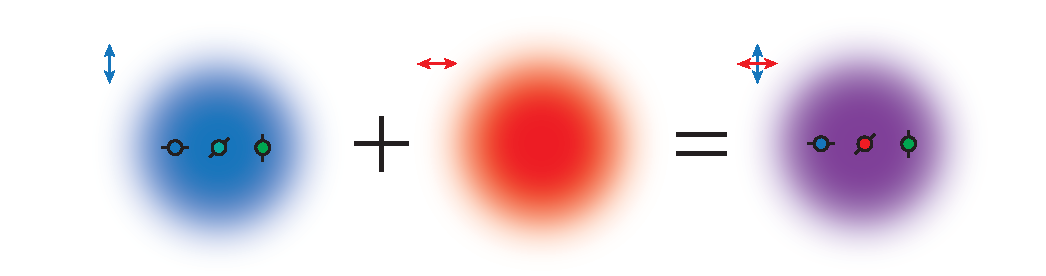
\includegraphics[width=\linewidth]{psted.ai}
	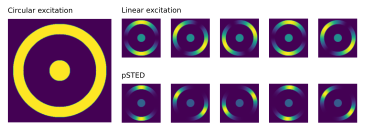
\includegraphics{psted_simulation.pdf}
	\caption{
		\textbf{Top:} Illustration of the working principle of pSTED. The arrows outside indicate the polarisation of the laser light. The circles represent fluorophores with their transition dipole moment indicated by a line. The orthogonal polarisation of the depletion beam suppresses fluorescence of the fluorophore oriented at \ang{45}.
		\textbf{Middle:} A simulation of pSTED compared to other excitation schemes on a sample consisting of a non-polarised disk and a radially polarised ring, where the excitation polarisation goes from \ang{0} to \ang{180}.
		\textbf{Bottom:} Simulation of a grid of superimposed fibres, where the fluorophores are aligned with the fibre. If the fibre spacing is below the spatial resolution, then pSTED can show the presence of two different orientations. The excitation polarisation in this figure goes from \ang{-20} to \ang{+20}.
	}
	\label{fig:psted principle}
\end{figure}

What follows is strongly inspired by Dyba et al.~\cite{Dyba2005}. Let $ \vb{x} = (x, y, z)$ be the spatial coordinates, $ \theta $ be an angle with the $ x $ axis in the $ xy $ plane (ranging from $ 0 $ to $ 2\pi$) and $ \phi $ be an angle with the $ z $ axis in the $ xz $ plane (ranging from $ -\pi $ to $+\pi$). We can also introduce a generalised coordinate $ \vb{y} = (\vb{x}, \theta, \phi) $ for a more convenient notation.
Let the fluorophore population be described by the density $ \rho(\vb{y}) $. This function is normalised such that its integral is equal to the number of fluorophores. For example, a single fluorophore at the origin, whose transition dipole points in the $ x $ direction with no out-of-plane tilt would be described by the Dirac delta distribution $ \rho_0 = \delta(\vb{y}) $, defined as follows:
\begin{gather}
	\delta(\vb{y}) = 0 \qq{if} y\neq0, \\
	\int f(\vb{y})\delta(\vb{y}-\vb{y}_0) \dd{\vb{y}} = f(\vb{y}_0).
\end{gather}

The excitation beam is described by the electric field amplitude $ \vb{E}_\exc $, polarised along $ \theta_\exc $, and analogous for the depletion beam. Like \autoref{eq:convolution}, the emission intensity measured when the laser is focused on $ \vb{x} $ and polarised along $ \theta $, $ \phi $ is now a convolution integral where we also have to integrate over the angles $ \theta $ and $ \phi $ like
\begin{equation}
	\begin{aligned}
		I_\emm 
			&= A \int 
				\sigma_\exc \abs{\unit{n}_{\theta'\phi'} \cdot \vb{E}_\exc(\vb{x}-\vb{x}')}^2 
				\rho(\vb{y}') 
				\dd{\vb{y}'} \\
			&= \int 
				\sigma_\exc I_\exc(\vb{x}'-\vb{x}) \abs{\unit{n}_{\theta'\phi'}\unit{n}_{\theta\phi}}^2
				\rho(\vb{y}') 
				\dd{\vb{y}'}
	\end{aligned}
\end{equation}
where $ \unit{n}_{\theta\phi} $ is a unit vector pointing in the direction of $ (\theta, \phi) $ and $ A = \epsilon_0c/2 $. $ \epsilon_0 $ is a constant denoting the vacuum permittivity. The dot product can be expressed as
\begin{equation}
	\abs{\unit{n}_{\theta'\phi'}\unit{n}_{\theta\phi}}^2 = \cos^2(\theta-\theta') \cos^2(\phi-\phi'),
\end{equation}
so we can write that equation as a convolution product like
\begin{gather}
	I_\emm = (\rho*h_\exc)(\vb{y}),\qq{where} \\
	h_\exc(\vb{y}) = \sigma_\exc I_\exc(\vb{x}) \cos^2\theta\cos^2\phi.
\end{gather}
If we have a constant laser intensity $ I_\exc $ that is polarised along $ \theta_\exc $ without any out-of-plane polarisation, this reduces to
\begin{equation}
	I_\emm = \sigma_\exc I_\exc \cos^2\theta_\exc
\end{equation}
for the distribution $ \rho_0 $. $ I_\emm $ is maximal when the excitation polarisation is in the $ x $ direction, as expected. From this equation, we can derive the same angular resolution as before, but with more rigour.

Now, we need to include the effect of the polarised depletion field, which amounts to adding an exponential factor under the integral
\begin{equation}
	I_\emm = A \int
		\sigma_\exc \abs{\unit{n}_{\theta'\phi'} \cdot \vb{E}_\exc(\vb{x}-\vb{x}')}^2  
		\exp(-\sigma_\dep \abs{\unit{n}_{\theta'\phi'} \cdot \vb{E}_\dep(\vb{x}-\vb{x}')}^2)
		\rho(\vb{y}') 
		\dd{\vb{y}'}.
	\label{eq:psted integral}
\end{equation}
In essence, this is equivalent to multiplying the kernel $ h_\exc $ with the function $ \eta $
\begin{equation}
	h(\vb{y}) = h_\exc(\vb{y}) \cdot \eta(\vb{y}) \qq{, where} \eta(\vb{y}) = \exp(-\sigma_\dep I_\dep(\vb{x}) \sin^2 \theta),
	\
\end{equation}
which assumes both electric fields are orthogonally polarised and confined to the $ xy $ plane.

\begin{figure}
	\centering
	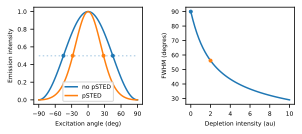
\includegraphics{pol_psf_width.pdf}
	\caption{
		\textbf{Left:} Narrowing of the fluorophore response as a result of a depletion field (of intensity $ I_\dep=2 $, as compared to the right pane). \textbf{Right:} The FWHM angular resolution $ d_\theta $ as a function of depletion intensity.
	}
	\label{fig:pol psf width}
\end{figure}

Now, we can calculate the angular resolution of this method. With a bit of algebra, it can be shown that the FWHM resolution equals
\begin{equation}
	d_\theta = 2\arccos\sqrt\frac{\mathcal{W}(k e^{k}/2)}{k},
\end{equation}
where $ k = \sigma_\dep I_\dep $ and $ \mathcal{W}(\cdot) $ denotes the Lambert W-function, the inverse of the function $ f(x) = xe^x $. As expected, $ d_\theta=\ang{90} $ for $ I_d=0 $. For other values of $ I_d $, the resolution is plotted in \autoref{fig:pol psf width}.

In an experiment, one could account for depolarising effects such as rotational diffusion, energy transfer, et cetera. That is not necessary at this point, but could be easily modelled by convolving $ \eta $ with a depolarisation kernel $ \delta $. This kernel would be a probability distribution that quantifies how much a dipole can move and rotate between absorption and interaction with the depletion beam. It is also possible to model polarised detection with
\begin{equation}
	h = h_\exc \cdot (\eta * \delta_1) \cdot (h_\mathit{det} * \delta_2).
\end{equation}





\subsection{Implementation}
\label{sec:psted implementation}

The system was not set up for tuning the depletion polarisation. Instead, the STED polarisation is always circular, and this is ensured by a set of two fixed waveplates: a QWP and a HWP (refer to \autoref{fig:layout} and the description of the STED module in that section). 

To control the polarisation of the depletion beam, I first had to linearise the polarisation by compensating for the QWP in the beam path. That can be done by placing a QWP in the pSTED module in \autoref{fig:layout}, since
\begin{equation}
	S_\qwp(\phi)S_\hwp(0)S_\qwp(-\phi) = R(2\phi).
\end{equation}
When the quarter-wave plates are aligned like that, this system simply rotates the polarisation by a fixed angle. This means that adding a HWP before this setup suffices to get full control over the polarisation angle of the depletion beam.

\begin{figure}
	\centering
	\includegraphics[height=.35\linewidth]{psted optics 1.jpg}%
	\hfill%
	\includegraphics[height=.35\linewidth]{psted optics top.jpg}
	\caption{
		The new pSTED optics. The rotational stage holds a HWP and a stationary QWP is mounted on a cage system. To take these optics out of the microscope, only the screw that holds the foot needs to be removed.
	}
	\label{fig:psted optics photo}
\end{figure}

In practice, the first step was to mount these two new waveplates in the beam path. They were mounted right after the SLM on an easily removable foot, see \autoref{fig:psted optics photo}. This way, conventional STED and polarisation-resolved STED are both easily performed. The HWP was mounted inside a rotational stage and the QWP in a cage system attached to the rotational stage, such that it is always aligned with the laser beam, but that its rotational angle is fixed. The first step was to find the angle of the QWP that maximised the linearity of the light polarisation at the sample. This was done by placing a polariser and a power meter at the sample and rotating them to characterise the polarisation of the depletion beam. I did this a couple of times, from which we concluded that the optimal angle for the QWP was \ang{15}. Next, I had to find the angle of the HWP at which the depletion beam is vertically polarised. In that position, the depletion beam has a polarisation parallel to the excitation lasers (at \ang{0}). This turned out to be \ang{38.5} (or equivalently $\ang{38.5}+\ang{180}=\ang{218.5}$). See \autoref{fig:psted hwp offset}. At a linearity of $ I_{max}/I_{min} = 5.47 $, the polarisation of the linearised pSTED beam is comparable in quality to the 640 laser (see \autoref{tab:laser polarisation}). Note that the HWP angle $ \theta_\hwp $ must satisfy
\begin{equation}
	\theta_\hwp = \ang{218.5} - \theta/2
\end{equation} 
to achieve a linear polarisation along $ \theta $ in the sample plane.

\begin{figure}
	\centering
	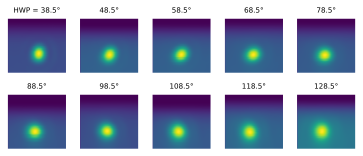
\includegraphics{psted_psfs.pdf}
	\caption{
		Depletion PSF as a function of beam polarisation. The figure titles indicate the angle of the new HWP. The shown images are recentred on the pixel with the highest intensity to correct for displacement. Scale bars 100~nm.
	}
	\label{fig:psted psfs}
\end{figure}

Now that we have control over the beam polarisation, we can check how the added waveplates influence the PSF. In \autoref{fig:psted psfs}, the PSF is shown for different polarisation directions. There are several conclusions we can draw from this data.  Firstly, the PSF is not radially symmetric any longer, even though the SLM was set to Gaussian mode. (This is easy to do. It only requires removing the donut-generating pattern on the SLM.) In particular, the ellipse orientation is parallel to the light polarisation, so we see the PSF rotating as we change the polarisation (see also \autoref{fig:psted psf orientation and power}). This can be explained by the fact that lenses interacts differently with light polarised along different directions \cite{Egner2020}. This is the reason one should only use linearly polarised excitation light when performing polarisation microscopy.

Other effects of the polarisation include the following: the intensity of the depletion beam varies as a function of the polarisation angle. See \autoref{fig:psted psf orientation and power}. This is probably due to linear dichroism present in the optical elements between the waveplates and the sample. This is not a surprising result, but should be accounted for during either image acquisition or analysis. Furthermore, the maximum of the PSF moves a little: up to roughly 100~nm from its mean position (\autoref{fig:psted displacement}). Fortunately, this is quite a bit below the diffraction limit for 775 nm light, i.e.~around 400 nm, so the effect will be rather small.

\section{Samples}
\label{sec:samples}

During the project, samples were very generously provided by research groups led by Pontus Nordenfelt and Vinay Swaminathan (%Division of Infection Medicine, 
Faculty of Medicine, Lund University).

Results of the cell sample shown in the experimental section contain a human cell line infected with bacteria of the Yersinia genus. Stainings present are: DAPI (nucleus), GFP (bacteria) and SiR-actin. SiR-actin is an organic molecule (silicon-rhodamine) rigidly linked to an actin monomer. This dye is perfect for our setup, as SiR can be excited at 664~nm and has a sufficient absorption cross-section at 775~nm to perform STED. In addition, the fact that it is rigidly bound to the actin cytoskeleton means the light it emits is strongly polarised and reports on the actin filament orientation.

I also used two control samples for calibration measurements. The first is a sample of reflective gold colloids, which were used to image the laser point spread functions. The second contains larger Tetraspec fluorescent beads (Invitrogen).